% Created by tikzDevice version 0.6.2-92-0ad2792 on 2013-04-07 23:43:57
% !TEX encoding = UTF-8 Unicode
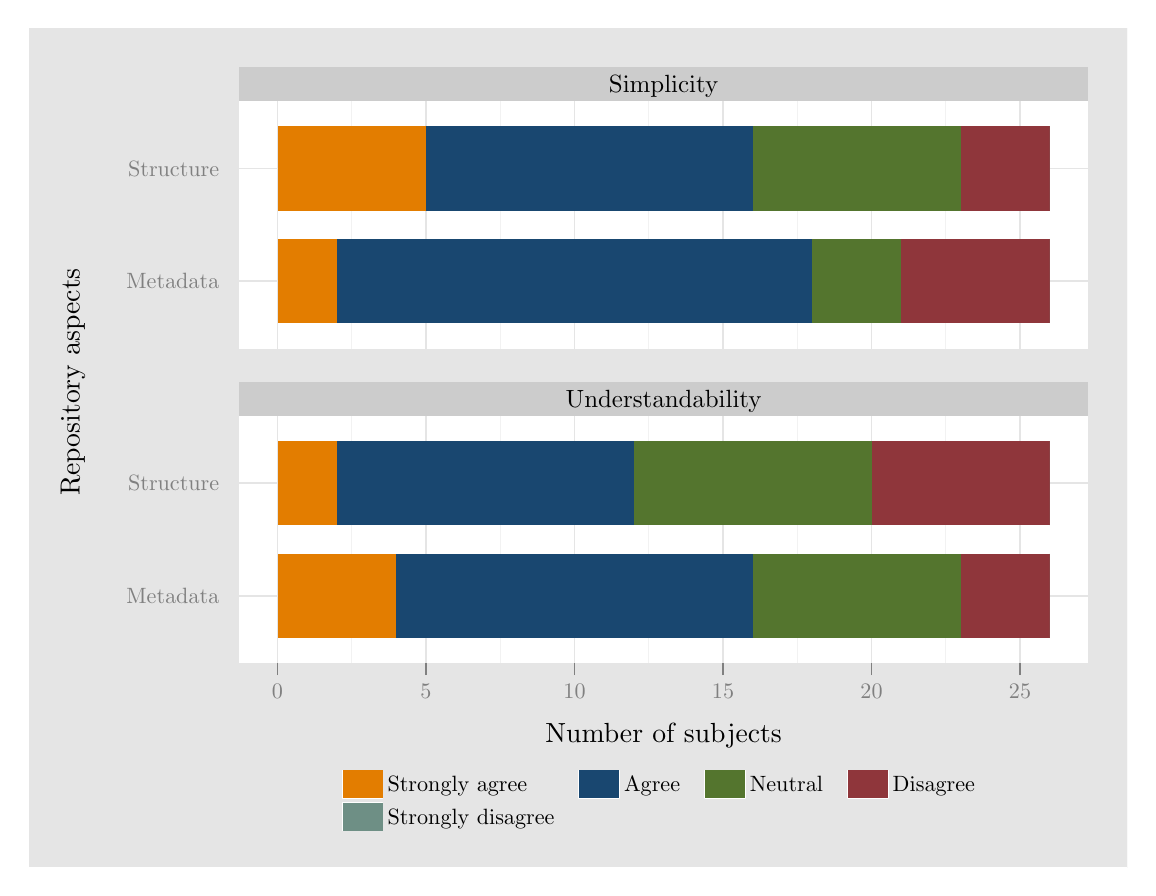
\begin{tikzpicture}[x=1pt,y=1pt]
\definecolor[named]{fillColor}{rgb}{1.00,1.00,1.00}
\path[use as bounding box,fill=fillColor,fill opacity=0.00] (0,0) rectangle (397.48,303.53);
\begin{scope}
\path[clip] (  0.00,  0.00) rectangle (397.48,303.53);
\definecolor[named]{drawColor}{rgb}{1.00,1.00,1.00}
\definecolor[named]{fillColor}{rgb}{0.90,0.90,0.90}

\path[draw=drawColor,line width= 0.6pt,line join=round,line cap=round,fill=fillColor] (  0.00,  0.00) rectangle (397.48,303.53);
\end{scope}
\begin{scope}
\path[clip] ( 76.33,187.58) rectangle (383.26,277.09);
\definecolor[named]{fillColor}{rgb}{1.00,1.00,1.00}

\path[fill=fillColor] ( 76.33,187.58) rectangle (383.26,277.09);
\definecolor[named]{drawColor}{rgb}{0.95,0.95,0.95}

\path[draw=drawColor,line width= 0.3pt,line join=round] (117.11,187.58) --
	(117.11,277.09);

\path[draw=drawColor,line width= 0.3pt,line join=round] (170.77,187.58) --
	(170.77,277.09);

\path[draw=drawColor,line width= 0.3pt,line join=round] (224.43,187.58) --
	(224.43,277.09);

\path[draw=drawColor,line width= 0.3pt,line join=round] (278.09,187.58) --
	(278.09,277.09);

\path[draw=drawColor,line width= 0.3pt,line join=round] (331.75,187.58) --
	(331.75,277.09);
\definecolor[named]{drawColor}{rgb}{0.90,0.90,0.90}

\path[draw=drawColor,line width= 0.6pt,line join=round] ( 76.33,211.99) --
	(383.26,211.99);

\path[draw=drawColor,line width= 0.6pt,line join=round] ( 76.33,252.68) --
	(383.26,252.68);

\path[draw=drawColor,line width= 0.6pt,line join=round] ( 90.28,187.58) --
	( 90.28,277.09);

\path[draw=drawColor,line width= 0.6pt,line join=round] (143.94,187.58) --
	(143.94,277.09);

\path[draw=drawColor,line width= 0.6pt,line join=round] (197.60,187.58) --
	(197.60,277.09);

\path[draw=drawColor,line width= 0.6pt,line join=round] (251.26,187.58) --
	(251.26,277.09);

\path[draw=drawColor,line width= 0.6pt,line join=round] (304.92,187.58) --
	(304.92,277.09);

\path[draw=drawColor,line width= 0.6pt,line join=round] (358.58,187.58) --
	(358.58,277.09);
\definecolor[named]{fillColor}{rgb}{0.89,0.49,0.00}

\path[fill=fillColor] ( 90.28,196.74) rectangle (111.75,227.25);
\definecolor[named]{fillColor}{rgb}{0.10,0.28,0.44}

\path[fill=fillColor] (111.75,196.74) rectangle (283.45,227.25);
\definecolor[named]{fillColor}{rgb}{0.33,0.46,0.18}

\path[fill=fillColor] (283.45,196.74) rectangle (315.65,227.25);
\definecolor[named]{fillColor}{rgb}{0.56,0.21,0.23}

\path[fill=fillColor] (315.65,196.74) rectangle (369.31,227.25);
\definecolor[named]{fillColor}{rgb}{0.43,0.56,0.52}

\path[fill=fillColor] (369.31,196.74) rectangle (369.31,227.25);
\definecolor[named]{fillColor}{rgb}{0.89,0.49,0.00}

\path[fill=fillColor] ( 90.28,237.42) rectangle (143.94,267.93);
\definecolor[named]{fillColor}{rgb}{0.10,0.28,0.44}

\path[fill=fillColor] (143.94,237.42) rectangle (261.99,267.93);
\definecolor[named]{fillColor}{rgb}{0.33,0.46,0.18}

\path[fill=fillColor] (261.99,237.42) rectangle (337.11,267.93);
\definecolor[named]{fillColor}{rgb}{0.56,0.21,0.23}

\path[fill=fillColor] (337.11,237.42) rectangle (369.31,267.93);
\definecolor[named]{fillColor}{rgb}{0.43,0.56,0.52}

\path[fill=fillColor] (369.31,237.42) rectangle (369.31,267.93);
\end{scope}
\begin{scope}
\path[clip] ( 76.33, 73.81) rectangle (383.26,163.32);
\definecolor[named]{fillColor}{rgb}{1.00,1.00,1.00}

\path[fill=fillColor] ( 76.33, 73.81) rectangle (383.26,163.32);
\definecolor[named]{drawColor}{rgb}{0.95,0.95,0.95}

\path[draw=drawColor,line width= 0.3pt,line join=round] (117.11, 73.81) --
	(117.11,163.32);

\path[draw=drawColor,line width= 0.3pt,line join=round] (170.77, 73.81) --
	(170.77,163.32);

\path[draw=drawColor,line width= 0.3pt,line join=round] (224.43, 73.81) --
	(224.43,163.32);

\path[draw=drawColor,line width= 0.3pt,line join=round] (278.09, 73.81) --
	(278.09,163.32);

\path[draw=drawColor,line width= 0.3pt,line join=round] (331.75, 73.81) --
	(331.75,163.32);
\definecolor[named]{drawColor}{rgb}{0.90,0.90,0.90}

\path[draw=drawColor,line width= 0.6pt,line join=round] ( 76.33, 98.22) --
	(383.26, 98.22);

\path[draw=drawColor,line width= 0.6pt,line join=round] ( 76.33,138.91) --
	(383.26,138.91);

\path[draw=drawColor,line width= 0.6pt,line join=round] ( 90.28, 73.81) --
	( 90.28,163.32);

\path[draw=drawColor,line width= 0.6pt,line join=round] (143.94, 73.81) --
	(143.94,163.32);

\path[draw=drawColor,line width= 0.6pt,line join=round] (197.60, 73.81) --
	(197.60,163.32);

\path[draw=drawColor,line width= 0.6pt,line join=round] (251.26, 73.81) --
	(251.26,163.32);

\path[draw=drawColor,line width= 0.6pt,line join=round] (304.92, 73.81) --
	(304.92,163.32);

\path[draw=drawColor,line width= 0.6pt,line join=round] (358.58, 73.81) --
	(358.58,163.32);
\definecolor[named]{fillColor}{rgb}{0.89,0.49,0.00}

\path[fill=fillColor] ( 90.28, 82.97) rectangle (133.21,113.48);
\definecolor[named]{fillColor}{rgb}{0.10,0.28,0.44}

\path[fill=fillColor] (133.21, 82.97) rectangle (261.99,113.48);
\definecolor[named]{fillColor}{rgb}{0.33,0.46,0.18}

\path[fill=fillColor] (261.99, 82.97) rectangle (337.11,113.48);
\definecolor[named]{fillColor}{rgb}{0.56,0.21,0.23}

\path[fill=fillColor] (337.11, 82.97) rectangle (369.31,113.48);
\definecolor[named]{fillColor}{rgb}{0.43,0.56,0.52}

\path[fill=fillColor] (369.31, 82.97) rectangle (369.31,113.48);
\definecolor[named]{fillColor}{rgb}{0.89,0.49,0.00}

\path[fill=fillColor] ( 90.28,123.65) rectangle (111.75,154.16);
\definecolor[named]{fillColor}{rgb}{0.10,0.28,0.44}

\path[fill=fillColor] (111.75,123.65) rectangle (219.06,154.16);
\definecolor[named]{fillColor}{rgb}{0.33,0.46,0.18}

\path[fill=fillColor] (219.06,123.65) rectangle (304.92,154.16);
\definecolor[named]{fillColor}{rgb}{0.56,0.21,0.23}

\path[fill=fillColor] (304.92,123.65) rectangle (369.31,154.16);
\definecolor[named]{fillColor}{rgb}{0.43,0.56,0.52}

\path[fill=fillColor] (369.31,123.65) rectangle (369.31,154.16);
\end{scope}
\begin{scope}
\path[clip] (  0.00,  0.00) rectangle (397.48,303.53);
\definecolor[named]{fillColor}{rgb}{0.80,0.80,0.80}

\path[fill=fillColor] ( 76.33,277.09) rectangle (383.26,289.31);
\definecolor[named]{drawColor}{rgb}{0.00,0.00,0.00}

\node[text=drawColor,anchor=base,inner sep=0pt, outer sep=0pt, scale=  0.90] at (229.80,280.10) {Simplicity};
\end{scope}
\begin{scope}
\path[clip] (  0.00,  0.00) rectangle (397.48,303.53);
\definecolor[named]{fillColor}{rgb}{0.80,0.80,0.80}

\path[fill=fillColor] ( 76.33,163.32) rectangle (383.26,175.54);
\definecolor[named]{drawColor}{rgb}{0.00,0.00,0.00}

\node[text=drawColor,anchor=base,inner sep=0pt, outer sep=0pt, scale=  0.90] at (229.80,166.33) {Understandability};
\end{scope}
\begin{scope}
\path[clip] (  0.00,  0.00) rectangle (397.48,303.53);
\definecolor[named]{drawColor}{rgb}{0.50,0.50,0.50}

\node[text=drawColor,anchor=base east,inner sep=0pt, outer sep=0pt, scale=  0.80] at ( 69.22,209.24) {Metadata};

\node[text=drawColor,anchor=base east,inner sep=0pt, outer sep=0pt, scale=  0.80] at ( 69.22,249.92) {Structure};
\end{scope}
\begin{scope}
\path[clip] (  0.00,  0.00) rectangle (397.48,303.53);
\definecolor[named]{drawColor}{rgb}{0.50,0.50,0.50}

\node[text=drawColor,anchor=base east,inner sep=0pt, outer sep=0pt, scale=  0.80] at ( 69.22, 95.47) {Metadata};

\node[text=drawColor,anchor=base east,inner sep=0pt, outer sep=0pt, scale=  0.80] at ( 69.22,136.15) {Structure};
\end{scope}
\begin{scope}
\path[clip] (  0.00,  0.00) rectangle (397.48,303.53);
\definecolor[named]{drawColor}{rgb}{0.50,0.50,0.50}

\path[draw=drawColor,line width= 0.6pt,line join=round] ( 90.28, 69.54) --
	( 90.28, 73.81);

\path[draw=drawColor,line width= 0.6pt,line join=round] (143.94, 69.54) --
	(143.94, 73.81);

\path[draw=drawColor,line width= 0.6pt,line join=round] (197.60, 69.54) --
	(197.60, 73.81);

\path[draw=drawColor,line width= 0.6pt,line join=round] (251.26, 69.54) --
	(251.26, 73.81);

\path[draw=drawColor,line width= 0.6pt,line join=round] (304.92, 69.54) --
	(304.92, 73.81);

\path[draw=drawColor,line width= 0.6pt,line join=round] (358.58, 69.54) --
	(358.58, 73.81);
\end{scope}
\begin{scope}
\path[clip] (  0.00,  0.00) rectangle (397.48,303.53);
\definecolor[named]{drawColor}{rgb}{0.50,0.50,0.50}

\node[text=drawColor,anchor=base,inner sep=0pt, outer sep=0pt, scale=  0.80] at ( 90.28, 61.19) {0};

\node[text=drawColor,anchor=base,inner sep=0pt, outer sep=0pt, scale=  0.80] at (143.94, 61.19) {5};

\node[text=drawColor,anchor=base,inner sep=0pt, outer sep=0pt, scale=  0.80] at (197.60, 61.19) {10};

\node[text=drawColor,anchor=base,inner sep=0pt, outer sep=0pt, scale=  0.80] at (251.26, 61.19) {15};

\node[text=drawColor,anchor=base,inner sep=0pt, outer sep=0pt, scale=  0.80] at (304.92, 61.19) {20};

\node[text=drawColor,anchor=base,inner sep=0pt, outer sep=0pt, scale=  0.80] at (358.58, 61.19) {25};
\end{scope}
\begin{scope}
\path[clip] (  0.00,  0.00) rectangle (397.48,303.53);
\definecolor[named]{drawColor}{rgb}{0.00,0.00,0.00}

\node[text=drawColor,anchor=base,inner sep=0pt, outer sep=0pt, scale=  1.00] at (229.80, 45.27) {Number of subjects};
\end{scope}
\begin{scope}
\path[clip] (  0.00,  0.00) rectangle (397.48,303.53);
\definecolor[named]{drawColor}{rgb}{0.00,0.00,0.00}

\node[text=drawColor,rotate= 90.00,anchor=base,inner sep=0pt, outer sep=0pt, scale=  1.00] at ( 18.80,175.45) {Repository aspects};
\end{scope}
\begin{scope}
\path[clip] (  0.00,  0.00) rectangle (397.48,303.53);
\definecolor[named]{fillColor}{rgb}{0.90,0.90,0.90}

\path[fill=fillColor] (105.91,  9.15) rectangle (353.68, 39.41);
\end{scope}
\begin{scope}
\path[clip] (  0.00,  0.00) rectangle (397.48,303.53);
\definecolor[named]{drawColor}{rgb}{1.00,1.00,1.00}
\definecolor[named]{fillColor}{rgb}{1.00,1.00,1.00}

\path[draw=drawColor,line width= 0.6pt,line join=round,line cap=round,fill=fillColor] (113.79, 25.19) rectangle (128.24, 35.14);
\end{scope}
\begin{scope}
\path[clip] (  0.00,  0.00) rectangle (397.48,303.53);
\definecolor[named]{fillColor}{rgb}{0.89,0.49,0.00}

\path[fill=fillColor] (113.79, 25.19) rectangle (128.24, 35.14);

\path[] (113.79, 25.19) --
	(128.24, 35.14);
\end{scope}
\begin{scope}
\path[clip] (  0.00,  0.00) rectangle (397.48,303.53);
\definecolor[named]{drawColor}{rgb}{1.00,1.00,1.00}
\definecolor[named]{fillColor}{rgb}{1.00,1.00,1.00}

\path[draw=drawColor,line width= 0.6pt,line join=round,line cap=round,fill=fillColor] (199.26, 25.19) rectangle (213.72, 35.14);
\end{scope}
\begin{scope}
\path[clip] (  0.00,  0.00) rectangle (397.48,303.53);
\definecolor[named]{fillColor}{rgb}{0.10,0.28,0.44}

\path[fill=fillColor] (199.26, 25.19) rectangle (213.72, 35.14);

\path[] (199.26, 25.19) --
	(213.72, 35.14);
\end{scope}
\begin{scope}
\path[clip] (  0.00,  0.00) rectangle (397.48,303.53);
\definecolor[named]{drawColor}{rgb}{1.00,1.00,1.00}
\definecolor[named]{fillColor}{rgb}{1.00,1.00,1.00}

\path[draw=drawColor,line width= 0.6pt,line join=round,line cap=round,fill=fillColor] (244.68, 25.19) rectangle (259.13, 35.14);
\end{scope}
\begin{scope}
\path[clip] (  0.00,  0.00) rectangle (397.48,303.53);
\definecolor[named]{fillColor}{rgb}{0.33,0.46,0.18}

\path[fill=fillColor] (244.68, 25.19) rectangle (259.13, 35.14);

\path[] (244.68, 25.19) --
	(259.13, 35.14);
\end{scope}
\begin{scope}
\path[clip] (  0.00,  0.00) rectangle (397.48,303.53);
\definecolor[named]{drawColor}{rgb}{1.00,1.00,1.00}
\definecolor[named]{fillColor}{rgb}{1.00,1.00,1.00}

\path[draw=drawColor,line width= 0.6pt,line join=round,line cap=round,fill=fillColor] (296.32, 25.19) rectangle (310.77, 35.14);
\end{scope}
\begin{scope}
\path[clip] (  0.00,  0.00) rectangle (397.48,303.53);
\definecolor[named]{fillColor}{rgb}{0.56,0.21,0.23}

\path[fill=fillColor] (296.32, 25.19) rectangle (310.77, 35.14);

\path[] (296.32, 25.19) --
	(310.77, 35.14);
\end{scope}
\begin{scope}
\path[clip] (  0.00,  0.00) rectangle (397.48,303.53);
\definecolor[named]{drawColor}{rgb}{1.00,1.00,1.00}
\definecolor[named]{fillColor}{rgb}{1.00,1.00,1.00}

\path[draw=drawColor,line width= 0.6pt,line join=round,line cap=round,fill=fillColor] (113.79, 13.42) rectangle (128.24, 23.38);
\end{scope}
\begin{scope}
\path[clip] (  0.00,  0.00) rectangle (397.48,303.53);
\definecolor[named]{fillColor}{rgb}{0.43,0.56,0.52}

\path[fill=fillColor] (113.79, 13.42) rectangle (128.24, 23.38);

\path[] (113.79, 13.42) --
	(128.24, 23.38);
\end{scope}
\begin{scope}
\path[clip] (  0.00,  0.00) rectangle (397.48,303.53);
\definecolor[named]{drawColor}{rgb}{0.00,0.00,0.00}

\node[text=drawColor,anchor=base west,inner sep=0pt, outer sep=0pt, scale=  0.80] at (130.05, 27.41) {Strongly agree $\;\;$};
\end{scope}
\begin{scope}
\path[clip] (  0.00,  0.00) rectangle (397.48,303.53);
\definecolor[named]{drawColor}{rgb}{0.00,0.00,0.00}

\node[text=drawColor,anchor=base west,inner sep=0pt, outer sep=0pt, scale=  0.80] at (215.52, 27.41) {Agree $\;\;$};
\end{scope}
\begin{scope}
\path[clip] (  0.00,  0.00) rectangle (397.48,303.53);
\definecolor[named]{drawColor}{rgb}{0.00,0.00,0.00}

\node[text=drawColor,anchor=base west,inner sep=0pt, outer sep=0pt, scale=  0.80] at (260.94, 27.41) {Neutral $\;\;$};
\end{scope}
\begin{scope}
\path[clip] (  0.00,  0.00) rectangle (397.48,303.53);
\definecolor[named]{drawColor}{rgb}{0.00,0.00,0.00}

\node[text=drawColor,anchor=base west,inner sep=0pt, outer sep=0pt, scale=  0.80] at (312.58, 27.41) {Disagree $\;\;$};
\end{scope}
\begin{scope}
\path[clip] (  0.00,  0.00) rectangle (397.48,303.53);
\definecolor[named]{drawColor}{rgb}{0.00,0.00,0.00}

\node[text=drawColor,anchor=base west,inner sep=0pt, outer sep=0pt, scale=  0.80] at (130.05, 15.64) {Strongly disagree $\;\;$};
\end{scope}
\end{tikzpicture}
